\chapter{Especificação da aplicação} \label{CHP:APP}%%
 
\section{Visão geral}
Com o intuito de demonstrar a aplicação em estudo com as áreas apresentadas nos capítulos \ref{CHP:TEO} e \ref{CHP:FUND}, foi idealizado um aplicativo com módulos \emph{Web} e \emph{Mobile}.
        Um \emph{quiz} é uma modalidade de jogo onde os jogadores têm por objetivo responder determinadas questões corretamente. Usualmente, \emph{quizzes} são usados em educação e entretenimento para medir grau de conhecimento e habilidades, como pensamento rápido e associação mental. Em modalidades mais competitivas, os \emph{quizzes} podem ter pontuações e, para competições em grupo, pode ter um vencedor (o participante com maior pontuação, por exemplo).
		
        %Conforme citado no capitulo \ref{fund},os aplicativos mais requisitados nos mercados de aplicativos móveis são de entretenimento e de jogos. Desse modo, idealizamos um sistema, composto de dois grandes módulos:
		O sistema é formado por dois grandes módulos:
\begin{itemize}
\item Sistema \emph{web}: nessa parte da aplicação, usuários podem gerenciar suas contas (metadados) e criar \emph{quizzes}. No momento da criação, tal usuário é denominado ``criador'', e recebe uma pontuação por participação nesse processo. Nesse sistema, também é possível consultar os resultados dos jogos (ou partida) realizada sobre cada um dos \emph{quizzes};
\item Sistema \emph{mobile}: nessa parte da aplicação, que está sobre as plataformas \emph{Android} e \emph{iOS} de forma nativa, o usuário (agora denominado ``jogador''), pode baixar os \emph{quizzes} de seu interesse para seu dispositivo e jogar, enviando seu resultado no final para ser consultado posteriormente por um criador.
\end{itemize} 
Tal sistema pode ser usado com duas finalidades básicas: entreter e realizar pesquisas. Na primeira forma, perguntas de conhecimento são criadas e jogadas casualmente, com o intuito de acertar uma pergunta. Na segunda forma, pode ser usada como uma enquete, onde o objetivo não é acertar uma determinada resposta, mas sim informar qual das opções corresponde a uma verdade do usuário.
 
\section{Requisitos}
 
\subsection{Requisitos funcionais}
Os requisitos funcionais definem ações que um sistema ou componente devem ser capazes de executar, sem levar em consideração restrições físicas. Para a aplicação iQuizzer, temos os seguintes requisitos:
\begin{itemize}
\item Gerenciamento de \emph{quiz}: a aplicação deve fornecer meios para que o dono do \emph{quiz} possa inserir, modificar ou apagar dados relativos ao \emph{quiz}, as perguntas pertencentes a ele e as respostas pertencentes a cada pergunta;
\item Sistema de pontos: a aplicação deve adicionar pontos a cada \emph{quiz} ou pergunta inseridos por um criador de \emph{quiz}. Além disso, deve adicionar pontos relativos a cada jogo, desde que o modo de jogo do \emph{quiz} executado permita acumular pontos;
\item Gerenciamento de resultados: a aplicação deve permitir ao criador visualizar as respostas marcadas (acertos e erros, a depender do modo de jogo), de cada jogador, ao seu \emph{quiz};
\item Gerenciamento de conta: a aplicação deve fornecer meios para que o usuário possa criar e apagar sua conta. Além disso, deve permitir ao usuário modificar seus dados cadastrais.
\end{itemize} 
 
\subsection{Requisitos não-funcionais}\label{SEC:RNF}
Os requisitos não-funcionais especificam alguns fatores relacionados ao uso da aplicação, como desempenho, usabilidade, confiabilidade, entre outros. Esses requisitos podem constituir restrições aos requisitos funcionais, pois são características mínimas de um software de qualidade, ficando a cargo do desenvolvedor optar ou não por atender esses requisitos.  Para a aplicação iQuizzer, temos os seguintes requisitos:
\begin{itemize}
\item Interatividade: a aplicação deve exigir interação do usuário, de maneira rápida e intuitiva. Atividades básicas não podem demandar muitas interações;
\item Confiabilidade: a aplicação não pode apresentar erros durante a execução. O sistema móvel deve prever situações de perda de conexão e situações de estouro de memória;
\item Integridade e privacidade dos dados: toda a informação trocada entre o sistema móvel e o sistema \emph{web} deve ser mantidas de maneira integra. Além disso, os dados do sistema \emph{web} só podem ser visualizados caso haja autorização para isso, ou seja, devem existir autenticação e tokens de autenticação.
\end{itemize} 
\section{Casos de uso}
O diagrama de casos de uso fornece um modo de descrever o sistema e suas interações com o mundo exterior, representando uma visão de alto nível da funcionalidade do sistema mediante uma requisição do usuário.
 
\begin{figure}[H]
  % Requires \usepackage{graphicx}
  \centering
  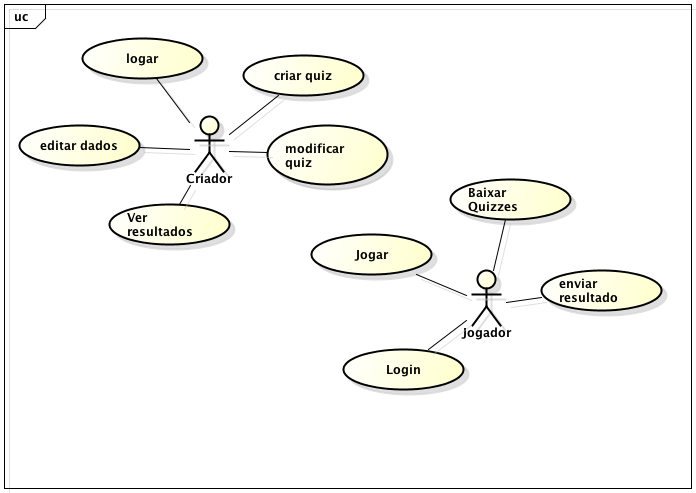
\includegraphics[scale =0.6]{figs/casos_de_uso.png}\\
  \caption{ Diagrama de casos de uso para ``criador'' e ``jogador'' }
  \label{FIG:Form_Factor}
\end{figure} 
 
 
\section{Diagrama de classes}\label{SEC:MER}
 
	Diagrama de classes é uma representação da estrutura e relações das classes que servem de modelo para objetos. Com ela, é possível ter uma visão rápida das classes do sistema, de modo a ajudar na implementação do modelo (M do \ac{MVC}) da aplicação. Além disso, é a base para construção dos diagramas de comunicação, sequência e estados.

        Nesse diagrama, estão representadas as tabelas básicas para o funcionamento da aplicação iQuizzer. Existem três entidades principais, a saber:
\begin{itemize}
\item Usuário: é a classe que representa o jogador e o criador do \emph{quiz}. Além das informações básicas, como nome e email, estão guardadas informações para login (nome de usuário, senha) e a pontuação (de criador e jogador).
\item Quiz: é a classe que representa um \emph{quiz}. Hierarquicamente, um \emph{quiz} possui um número ilimitado de perguntas únicas, e uma pergunta possui um número ilimitado de respostas únicas. Cada \emph{quiz} possui um modo de jogo, que indica se é um \emph{quiz} de perguntas arbitrárias, em sequência, com tempo, etc., e um número máximo de perguntas a ser jogado por partida.
\item Jogo: essa classe representa cada uma das partidas (jogos) que foram realizadas por cada jogador no sistema móvel. Cada jogo possui uma quantidade de resultados, correspondente ao número máximo de perguntas do \emph{quiz} jogado.
\end{itemize} 
 
\begin{figure}[H]
  % Requires \usepackage{graphicx}
  \centering
  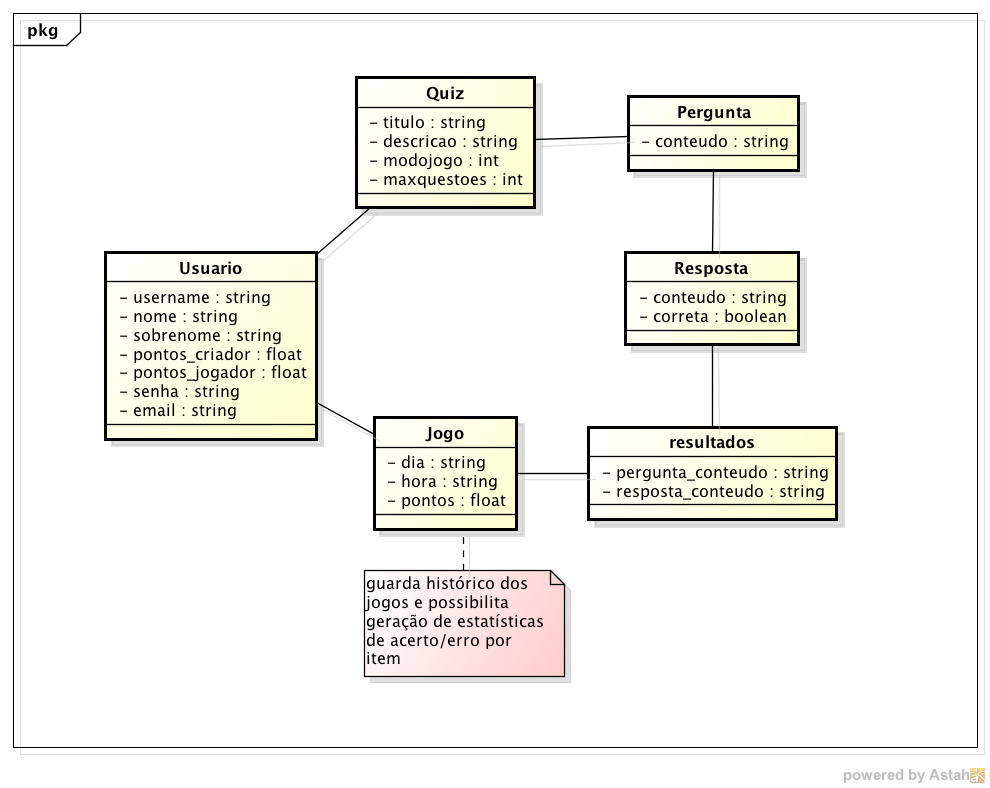
\includegraphics[scale =0.55]{figs/MER_web.png}\\
  \caption{ Diagrama de entidades }
  \label{FIG:Form_Factor2}
\end{figure}
